
\section{Introduction}

Canonical correlation analysis (CCA) is a well-known statistical approach
for multivariate analysis of two datasets~\citep{Hotelling1936}. In the
context of large-scale genomic and multi-omic analyses, CCA can prove useful
in identifying relationships amongst complex data, for example single
nucleotide polymorphisms (SNPs) and gene expression levels. Approaches
that consider one SNP at a time together with multiple phenotypes have
been shown to increase power to detect QTLs over the simpler but commonly
utilised single-SNP/single-phenotype approach~\citep{Ferreira2009,Inouye2012},
particularly when analysing correlated phenotypes that are modulated by the
same genetic variants.

Analysis of multiple SNPs simultaneously is an attractive extension of
the single-SNP multiple-phenotype approach, however, standard CCA is
not well-defined when the number of samples is lower than the number
of SNPs or phenotypes ($n{<}\min\{p, m\}$).  One solution is Sparse
CCA (SCCA)~\citep{Witten2009cshort,Witten2009bshort,Parkhomenko2009},
an $L_1$-penalised variant of CCA which allows for tuning the number of
variables that effectively contribute to the canonical correlation, thus
making the problem well-defined. Owing to the induced sparsity, SCCA can
be useful for identifying a small subset of SNPs and a small subset of the
phenotypes exhibiting strong correlations.  However, the rapidly increasing
size and coverage of genotyping arrays (exacerbated by genotype imputation),
together with the availability of large phenotypic datasets (transcriptomic,
metabolomic, and others; e.g., \citet{Bartel2015,TheGTExConsortium2015}),
makes it challenging to perform such analyses using existing tools.

We have developed an efficient implementation of SCCA that is
capable of analysing genome-wide SNP datasets (1 million SNPs
or more) together with thousands of phenotypes, as part of the tool
\texttt{flashpca}~\citep{Abraham2014}. The tool is implemented in \textsf{C++}
using the Eigen~3 numerical library~\citep{eigenweb}, as well as an \textsf{R}
interface (package \texttt{flashpcaR}) based on RcppEigen~\citep{Bates2013}.

Here, we compare the SCCA implementation in \texttt{flashpcaR} and
\texttt{flashpca} with a widely-used implementation (\texttt{PMA},
by~\citet{Witten2013short}), and demonstrate the substantial improvements
in speed of our tool, allowing for large analyses to be performed rapidly.

\vspace*{-12pt}
\begin{methods}
\section{Methods}

In standard CCA, we assume that we have two matrices $\mathbf{X}$ ($n \times p$)
and $\mathbf{Y}$ ($n \times m$), measured for the same $n$ samples.
We further assume that both $\mathbf{X}$ and $\mathbf{Y}$ have been
column-wise standardised (zero mean, unit variance).  For a single pair of 
canonical variables $a$ and $b$, CCA involves solving the problem
\vspace*{-10pt}
\begin{align}
\argmax_{a,b} & \frac{a^T \s_{XY} b}{\sqrt{a^T \s_{XX} a \; b^T \s_{YY} b}},
\label{eqn:cca}
\vspace*{-10pt}
\end{align}
where $\s_{XX}$ and $\s_{YY}$ are the covariance matrices of
$\mathbf{X}$ and $\mathbf{Y}$, respectively, and $\s_{XY}$ is the
covariance matrix of $\mathbf{X}$ and $\mathbf{Y}$. The solution is given by
the singular value decomposition (SVD) of $\s_{XX}^{-1/2} \s_{XY}
\s_{YY}^{-1/2}$, with $a = \s_{XX}^{-1/2} u_1$ and $b =
\s_{YY}^{-1/2} v_1$, where $u_1$ and $v_1$ are the first left and right
singular vectors, respectively.

SCCA is typically used for high-dimensional data, where a useful assumption is that
the columns of $\mathbf{X}$ and $\mathbf{Y}$ are uncorrelated,
i.e., $\s_{XX}=\s_{YY}=\mathbf{I}$~\citep{Parkhomenko2009},
hence, $a = u$ and~$b = v$. Thus, SCCA involves solving another form of CCA,
\vspace*{-6pt}
\begin{align}
\argmax_{u,v} &  \quad u^T \s_{XY} v \notag \\
 & \mbox{s.t. } ||u||_2^2=1, ||v||_2^2 = 1, ||u||_1 \le s_u, ||v||_1 \le s_v,
\label{eqn:scca}\vspace*{-10pt}
\end{align}
where $u$ and $v$ are the left and right canonical vectors, respectively, and
$s_u$ and $s_v$ are constraints on the $L_1$ norms of these canonical vectors.

The problem can be converted into the penalised (Lagrangian) form, making it
solvable using iterative soft-thresholding~\citep{Parkhomenko2009}, which we
employ here.  Unlike standard CCA, SCCA is well-defined even when $n{<}\min
\{p, m\}$, and induces sparse canonical vectors, depending on the choice of
$L_1$ penalties (higher penalties lead to higher sparsity). The optimal set
of penalties can be found via cross-validation: the data (both $\mathbf{X}$
and $\mathbf{Y}$) are split into training and test sets, SCCA is run on
the training set $(\mathbf{X}_{\mbox{train}}, \mathbf{Y}_{\mbox{train}})$
using a 2D grid of penalties, and the pair of penalties that produce the
highest correlations in the test set, $\mbox{Cor}(\mathbf{X}_{\mbox{test}}
u, \mathbf{Y}_{\mbox{test}} v)$, are selected.  Optionally, a new model may
be fitted to the entire data using these penalties.

%\enlargethispage{6pt}

\end{methods}

\begin{figure}[!tpb]
\centerline{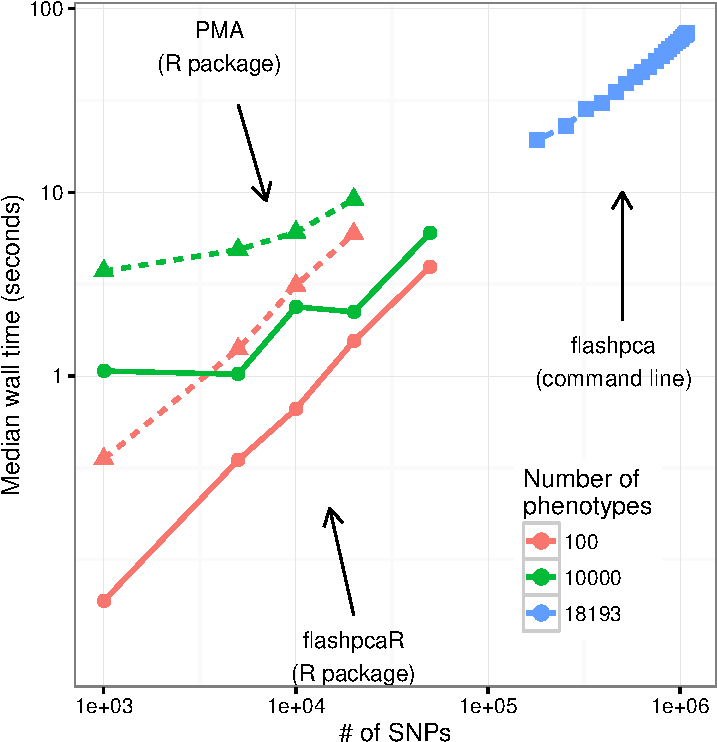
\includegraphics[width=\figwidthp\textwidth]{scca_timing-crop.pdf}}
\caption{
Timing (median of 30 runs) of SCCA implemented in (i) the \texttt{flashpcaR}
(\textsf{R} package) and (ii) \texttt{flashpca} (stand-alone commandline tool),
compared with \texttt{PMA}, using subsets of the HapMap3 dataset with gene
expression levels as phenotypes. The stand-alone \texttt{flashpca} timing
includes data loading into memory.
}
\label{fig:01}
\end{figure}

\section{Results}

We utilised the HapMap3 phase III genotypes~\citep{hapmap2010}, together with
gene expression data of~\nindiv individuals~\citep{Stranger2012}, with~1.4M
SNPs and~47,000 gene expression probes (out of which~21,800 probes were
analysed by~\citet{Stranger2012} and used in our analysis). After quality
control (see Supplementary Material) and taking the intersection of SNPs
across the populations, the data consisted of~\nindiv individuals, \nsnps
SNPs, and~\ngenes gene expression probes.

We first confirmed that \texttt{flashpcaR::scca} produced models comparable
with \texttt{PMA::CCA}, by comparing the results in cross-validation on HapMap3
genotypes together with simulated gene expression levels (Supplementary
Material).  Next, to further assesss the relative speed improvement using
real-world data, we used subsets of the HapMap3 genotypes and real gene
expression levels~\citep{Stranger2012} and compared the runtime of: (i)
\texttt{PMA::CCA} (\textsf{R} package), (ii) \texttt{flashpcaR::scca}
(\textsf{R} package), and (iii) \texttt{flashpca} (commandline tool).
Whereas both \texttt{PMA::CCA} and \texttt{flashpcaR::flashpca} are bound by
the memory limitations of \textsf{R}, the commandline tool \texttt{flashpca}
allows much larger analyses; hence we also ran larger analyses of increasing
size: chromosomes~1--2, 1--3, $\hdots$ , 1--22, up to all~\nsnps SNPs.
Figure~1\vphantom{\ref{fig:01}} shows that \texttt{flashpcaR::scca} was
$3\text{--}12\times$ faster than \texttt{PMA::CCA}, with an analysis
of 75,000 SNPs and~10,000 gene expression levels completing in~5s
and~50s, respectively. The commandline \texttt{flashpca} was faster
than \texttt{PMA::CCA} as well, and completed an analysis of~\nindiv
individuals, \nsnps SNPs and~\ngenes gene expression levels in median wall
time of ${\sim}47$s (including all overheads), using~${\sim}10$GiB of RAM.
Note that runtime for the commandline \texttt{flashpca} includes all steps
such as loading data into RAM, unlike the \textsf{R} version where the data
is pre-loaded into \textsf{R}.  Performing cross-validation over a grid of
penalties will increase these times considerably, in which case we recommend
parallelisation over several cores (Supplementary Material).\vspace*{-12pt}

\section{Conclusion}

\texttt{flashpca} provides a fast implementation of sparse canonial correlation
analysis, making it possible to rapidly analyse high dimensional datasets.
SCCA is available in the \textsf{R} package \texttt{flashpcaR}, which enables
analysis of metabolomic, transcriptomic, or any other quantitative set of
measurements. The commandline version is targeted at SNP/phenotype data,
enabling large QTL analyses of~${>}1$ million SNPs and thousands of phenotypes,
that would otherwise be too large to fit within \textsf{R}.\vspace*{-12pt}

\section*{Funding}

This work has been supported by the NHMRC (grant no.~1062227). GA was supported
by an NHMRC Early Career Fellowship (no.~1090462). MI was supported by a
Career Development Fellowship co-funded by the NHMRC and Heart Foundation
(no.~1061435).\vspace*{-12pt}

%\bibliographystyle{natbib}
%\bibliography{paper}

%\end{document}

